% Use the article doc class, with an 11 pt basic font size
%\documentclass[11pt, a4paper, draft]{article}
\documentclass[11pt, a4paper]{article}
% Nice citations
\usepackage{natbib}
% Set margins
\usepackage[margin=2.5cm]{geometry}
% Multilingual support
\usepackage[english]{babel}
% Nice mathematics and Left-right harpoons for kinetic equations
\usepackage{amsmath,mathtools}
% Control over maketitle
\usepackage{titling,titlesec}
% Ability to use colour in text
\usepackage[usenames]{color}
\definecolor{grey}{rgb}{0.6, 0.6, 0.63}
\definecolor{black}{rgb}{0, 0, 0}
% For the \degree symbol
\usepackage{textcomp,gensymb}
% Allow includegraphics and wrapped figures
\usepackage{graphicx,wrapfig,subfigure}
\usepackage[outercaption]{sidecap}
\usepackage{csquotes}
% For full page figures:
%\usepackage[CaptionAfterwards]{fitpage}

%% Trick to define a language alias and permit language = {en} in the .bib file.
% From: http://tex.stackexchange.com/questions/199254/babel-define-language-synonym
\usepackage{letltxmacro}
\LetLtxMacro{\ORIGselectlanguage}{\selectlanguage}
\makeatletter
\DeclareRobustCommand{\selectlanguage}[1]{%
  \@ifundefined{alias@\string#1}
    {\ORIGselectlanguage{#1}}
    {\begingroup\edef\x{\endgroup
       \noexpand\ORIGselectlanguage{\@nameuse{alias@#1}}}\x}%
}
\newcommand{\definelanguagealias}[2]{%
  \@namedef{alias@#1}{#2}%
}
\makeatother
\definelanguagealias{en}{english}
\definelanguagealias{eng}{english}
%% End language alias trick

%% Any aliases here
\newcommand{\mb}[1]{\mathbf{#1}} % this won't work?
% Emphasis and bold.
\newcommand{\e}{\emph}
\newcommand{\code}[1]{\textsf{#1}}
\newcommand{\dvrg}{\nabla\vcdot\nabla}
%% END aliases

% Custom font defs
% fontsize is \fontsize{fontsize}{linespacesize}
\def\authorListFont{\fontsize{11}{11} }
\def\corrAuthorFont{\fontsize{10}{10} }
\def\affiliationListFont{\fontsize{11}{11}\itshape }
\def\titleFont{\fontsize{14}{11} \bfseries }
\def\textFont{\fontsize{11}{11} }
\def\sectionHdrFont{\fontsize{11}{11}\bfseries}
\def\bibFont{\fontsize{10}{10} }
\def\captionFont{\fontsize{10}{10} }

% Caption font size to be small.
\usepackage[font=small,labelfont=bf]{caption}

% Make a dot for the dot product, call it vcdot for 'vector calculus dot'. Bigger than \cdot, smaller than \bullet.
\makeatletter
\newcommand*\vcdot{\mathpalette\vcdot@{.35}}
\newcommand*\vcdot@[2]{\mathbin{\vcenter{\hbox{\scalebox{#2}{$\m@th#1\bullet$}}}}}
\makeatother

\def\firstAuthorLast{James}
\def\Address{\\
\affiliationListFont Department of Psychology,\\
 \affiliationListFont  The University of Sheffield, Sheffield, UK \\
}
\def\corrAuthor{Seb James}
\def\corrAddress{Department of Psychology, The University of Sheffield,
  Western Bank, Sheffield, S10 2TP, UK}
\def\Authors{\authorListFont Sebastian~S.~James, Stuart~P.~Wilson  \Address}
%  \corrAuthorFont $^{*}$ Correspondence: {seb.james@sheffield.ac.uk}}

% If no page numbering wanted:
%\pagenumbering{gobble}

% A trick to get the bibliography to show up with 1. 2. etc in place of [1], [2] etc.:
\makeatletter
\renewcommand\@biblabel[1]{#1.}
\makeatother

% reduce separation between bibliography items if not using natbib:
\let\OLDthebibliography\thebibliography
\renewcommand\thebibliography[1]{
  \OLDthebibliography{#1}
  \setlength{\parskip}{0pt}
  \setlength{\itemsep}{0pt plus 0.3ex}
}

% Define title, empty date and authors
\title {
Time to stop; agent-based modelling of chemoaffinity with competition
}
\date{} % No date please
\author{\Authors}

%% END OF PREAMBLE

\begin{document}
%\setlength{\droptitle}{-1.8cm} % move the title up a suitable amount
\maketitle

\emph{We show that a true chemoaffinity model based on gradient-following (via receptor-ligand interactions) combined with receptor-ligand-mediated axonal repulsion, in which information is only transferred by nearest-neighbour interactions, can account for a broad range of experimental manipulations of the retinotectal system.}



%\begin{itemize}
%    \item Sperry's chemospecificity model is an influential theory of how axons from neurons that originate in one tissue can find their way to specific locations in a target tissue during early brain development.
%    \item A key component of the theory is that growing axons find their way into position by chemotaxis, i.e., by evaluating local information in gradients of gene expression that span the target tissue
%    \item Computational models have shown that in addition to chemotaxis, local competitive interactions between growing axons can account for a wide range of results from experiments in which the factors known to influence the growth of axons have been surgically or genetically manipulated
%    \item However, while such models have \emph{assumed} the effects of chemotaxis, the key assumption of the chemospecificity model, that axons sample and evaluate positional information only \emph{locally}, is yet to be tested directly.
%    \item Consider, for example, an important model by Goodhill \& Simpson, which shows how [a certain set of assumptions about the form of the] competition between axons can account for patterns of innervation in the developing tectum that result from ablating/rotating sections of the retina.
%    \item The formulation of this model includes a term that at every time-step moves the simulated axons in the direction of a pre-specified target location. Thus the model implicitly assumes a global supervisor, capable of evaluating the current state of each axon, computing a direction vector to correct its trajectory, and communicating that information to each axon.
%    \item This model was constructed primarily to establish the effects of competition, and to this end is elegantly formulated.
%    \item Nevertheless, the key assumptions of the chemospecificity model, and specifically the proposal that axons find their way via evaluating only local information (chemotaxis), are yet to be investigated directly.
%    \item The aim of the current study is therefore to construct a model that represents the assumptions of the chemospecificity model explicitly.
%    \item One advantage of such a model is that it can be used to investigate the sensitivity and robustness of local interactions in establishing topographic maps to various sources of noise.
%    \item Indeed, our simulation results show that the local mechanisms of axonal information-processing that are assumed by the chemospecificity model provide a remarkably robust solution to the problem of topographic map development.
%\end{itemize}

\section{Introduction}

% Could use chemoaffinity as a coverall theory, comprising chemospecificity and chemotaxis.

Sperry's chemoaffinity model is an influential theory of how axons from neurons that originate in one tissue can find their way to specific locations in a target tissue during early brain development \citep{sperry_reestablishment_1942,sperry_visuomotor_1943,sperry_chemoaffinity_1963}.
%
The central proposal of the theory is that growing axons find their location in a destination tissue by means of `labels of a cytochemical nature'.
The chemical affinity between labels in source and destination tissues allows axons to distinguish correct target locations from incorrect ones.
%
This key idea (called chemospecificity) does not, on its own, explain how an axon can find the correct \emph{direction} in which it should move to reach its target.
An additional component of Sperry's theory \citep{stevens_handbook_1950,sperry_problems_1955,sperry_chemoaffinity_1963} suggested that the axon could determine this direction by evaluating local information in gradients of gene expression spanning the target tissue, giving rise to chemotaxis of the axonal growth cones.

Much of Sperry's work was carried out on the retinotectal system, which is ideal for the study of ordered axonal development in fish, amphibia and birds, because in these animals, patterning of axons across the tectum is largely complete prior to the onset of neural activity (\textbf{find citation}).
In this system a two-dimensional map of the retina is developed on the surface of the optic tectum such that the axons from adjacent retinal ganglion cells (RGCs) find their way to adjacent locations on the tectum.
The retinotectal map is amenable to a number of surgical manipulations especially in amphibia, in which re-growth of the projection can be observed after surgical changes to the sensory apparatus (such as ablation or rotation of the retina) or the map substrate (the tectum).
This allowed Sperry and other researchers to carry out a wide range of experimental manipulations, the results of which informed the chemoaffinity theory.

In the 1990s, the theory of chemoaffinity and chemotaxis was given robust support by the discovery of the ephrin ligands and their receptors \citep{cheng_complementary_1995,drescher_vitro_1995} which have been shown to form into graded expression fields in the retina \citep{braisted_graded_1997}, tectum \citep{braisted_graded_1997,feldheim_genetic_2000} as well as in other sensory systems, such as the somatosensory system \citep{vanderhaeghen_mapping_2000}. % And sounds?
%
The Ephrin ligands have a clear effect on axonal outgrowth, as shown in-vitro \citep{cheng_complementary_1995,drescher_vitro_1995,hansen_retinal_2004} and by in-vivo \citep{frisen_ephrin-a5_1998,rodger_transient_2000,mann_topographic_2002,hindges_ephb_2002} studies.
Two classes of ephrins have been identified, labelled `A' and `B'.
Ephrin A and its receptors mediate a repulsive interaction which contributes to an ordering of RGC axons on the tectum along the rostral-caudal axis. Ephrin B acts on medial-lateral ordering with an attractive interaction.
Together, the ephrins are able to provide a coordinate system on the tectum to guide growing axons, but precisely how this positional information is used by axonal growth cones is not yet fully understood.

Quantitative models exploring axonal ordering were already in existence by the time of the discovery of the ephrins.
The importance of chemical gradients to biological processes was already well known from the study of slime moulds \citep{bonner_evidence_1947}.
Sperry himself discussed chemical gradients in relation to the problem of neuronal pathfinding \citep{sperry_problems_1955}, albeit qualitatively.
Some time after Sperry's active period, but before the ephrins were identified, \citet{gierer_development_1981,gierer_model_1983,gierer_directional_1987} made one of the few quantitative investigations of a gradient-based model of the retinotectal projection. He presented gradient following as a special case of a general class of \emph{potential models}.
In a potential model, the interactions between the properties of a growing axon originating from a location $\mathbf{u}$ on the retina and its environment at location $\mathbf{x}$ on the tectum set up some potential function, $p(\mathbf{x},\mathbf{u})$.
The axon then grows or moves to minimize $p$, which causes it to find its target location. This model successfully creates the wildtype map because each axon originates with a different $\mathbf{u}$ and has its minimum $p(\mathbf{x},\mathbf{u})$ in the correct target location.
This model forms a mathematical expression of Sperry's theory. Because it is quantitative, it allowed Gierer to identify two features of the theory: i) A \emph{pair} of opposing gradients is needed to form a potential function in one dimension (and \emph{two} pairs to create a 2D potential function). ii) Tectal or retinal ablation would require $p$ to be re-specified to reproduce the experimental results that fibres from an ablated retina will generate a map across the entire tectum and fibres from an intact retina will form a compressed map on an ablated tectum \citep{attardi_preferential_1963,schmidt_retinal_1978,schmidt_expansion_1978}.
Gierer addressed the second problem by introducing a form of competition between fibres, postulating that $p$ would accumulate locally at a rate proportional to the fibre density in that location and he noted that this was equivalent to a more direct fibre-fibre competition.
He demonstrated, in a one-dimensional computer simulation, that this form of competition would lead to the expected response to ablations \citep{gierer_model_1983}.

Gierer's simulations confirmed the validity of this basic idea, which we will refer to as \emph{differential chemotaxis}, for the problem of map formation with respect to a single spatial dimension \citep{gierer_model_1983,karbowski_model_2004}.
These models have also helped establish how competition between axons for space in the target tissue can additionally account for many of the known effects of surgical manipulation on map development.

Simulations of differential chemotaxis and axonal competition have recently been extended to investigate map development in two spatial dimensions, revealing how these two ingredients can give rise to realistic patterns of synaptic innervation \citep{james_modelling_2020}.
These models are formulated as systems of partial differential equations (PDE), and solved through numerical integration on an underlying lattice structure representing the target tissue.
In general, this approach makes mathematical analysis of system dynamics tractable, and as such PDE modelling has played a central r\^ole in the development of theories of pattern formation (see \citet{krause_modern_2021} for recent examples).
% Not sure about this:
However as the number of terms involved in PDEs necessarily grows large in systems representing differential chemotaxis, these systems quickly become impossible to analyse, making this potential advantage of such modelling redundant.
Additionally, the numerical simulation of a PDE system can become intractable, because each axonal projection must be represented by several state variables, each of which require solution across the entire spatial domain (which may consist of many thousands of elements).
% in james_modelling we did 41 projections. I found that trying to build a retinotectal system with about 100 projections was already intractable.

% But know we can motivate agent based modelling because *simulation* of PDEs for differential chemotaxis is intractable.
An alternative simulation approach is to treat each of $n$ axons as an agent that interacts with its environment and with the other $n-1$ axons.
The computation of such a system (see for example, \citet{simpson_simple_2011}) is dominated by the $O(n^2)$ axon-axon interactions and so a limit will be approached as $n\rightarrow \infty$.
We found that agent based simulations of $O(10^3)$ interacting axons can be achieved on a standard desktop computer whereas an equivalent PDE system would fail with about 100 axon projections.

\emph{PDEs too complex (can't do maths analysis), so need agent based. Can represent more biological detail and ask how that affects the systems level.}

\emph{List the questions that emerge from the discussion above}

\emph{Can Gierer model explain ALL the manipulations that S and G did?}

\emph{Allows us to make a specific representation of Gierer's model in which the receptor-ligand mechanism is elaborated.}

\textbf{xxxxxxxxxxxxxxx}

Computational models have shown that in addition to chemotaxis, local competitive interactions between growing axons can account for a wide range of results from experiments in which the factors known to influence the growth of axons have been surgically or genetically manipulated \citep{prestige_role_1975,simpson_simple_2011,suetterlin_target-independent_2014}.

However, while such models have \emph{assumed} the effects of chemotaxis, the key assumption of the chemoaffinity model, that axons sample and evaluate positional information only \emph{locally}, has yet to be tested directly.
%
Consider, for example, an important model by Goodhill \& Simpson, which shows how [a certain set of assumptions about the form of the] competition between axons can account for patterns of innervation in the developing tectum that result from ablating/rotating sections of the retina \citep{simpson_simple_2011}.
%
The formulation of this model includes a term that at every time-step moves the simulated axons in the direction of a pre-specified target location.
Thus the model implicitly assumes a global supervisor, capable of evaluating the current state of each axon, computing a direction vector to correct its trajectory, and communicating that information to each axon.
%
This model was constructed primarily to establish the effects of competition, and to this end is elegantly formulated.
%
Nevertheless, the key assumptions of the chemoaffinity model, and specifically the proposal that axons find their way by evaluating only local information (chemotaxis), are yet to be investigated directly.

The aim of the current study is therefore to construct a model that represents the assumptions of the chemotaxis model explicitly and to investigate how this mechanism behaves when combined with competitive interactions.

One advantage of such a model is that it can be used to investigate the sensitivity and robustness of local interactions in establishing topographic maps to various sources of noise.

Indeed, our results show that the local mechanisms of axonal information-processing that are assumed by the chemoaffinity model provide a remarkably robust solution to the problem of topographic map development.

\section{Results}
\subsection*{A model of chemotaxis and competition}

In an agent-based model of chemotaxis and competition, the position, $\mathbf{x}_t$, of each branch $b$ on a simulated tectum can be updated according to $\mathbf{x}_{t+1} = \mathbf{x}_{t} + \mathbf{M}$ with the movement vector $\mathbf{M}$ given by
\begin{equation} \label{e:mv2}
 \mathbf{M} = \mathbf{G} +  \mathbf{X} + \mathbf{B}.
\end{equation}
$\mathbf{G}$ is the movement due to the chemotaxis effect and $\mathbf{X}$ is the movement due to competitive interactions with other branches.
$\mathbf{B}$ is a movement applied close to the tissue boundary that ensures all branches remain within the tissue \citep{holt_target_1998}.

\citet{simpson_simple_2011} investigated a model of this form in which a `placeholder' provided a chemotaxis-like movement for $\mathbf{G}$ and a form for $\mathbf{X}$ was studied.
Their model, which successfully accounts for a wide range of experimental manipulations, found an $\mathbf{X}$ comprised of two components; a simple distance-based competition between \emph{all} branches ($\mathbf{C}$), along with an axon-axon interaction based on the relative levels of the receptor EphA expressed by each interacting axon ($\mathbf{I}$).
We asked i) if the placeholder mechanism for $\mathbf{G}$, in which a `global supervisor' informs each branch of the vector along which it should travel to approach its target, could be replaced by a true chemotaxis mechanism based on graded signalling molecule expression and ii) if the competition mechanism found by Simpson and Goodhill was the simplest possible mechanism that could explain all of the surgical and genetic manipulations accounted for by their model.

\subsection*{A gradient based model of chemotaxis}

We assumed a purely linear receptor binding model, and set the chemotactic movement vector of the branch $b$ at location $\mathbf{x}$ on the tectum to be

\begin{equation}\label{e:G}
\mathbf{G} = m_{\!_G}\,\sum_i^N F_i\,r_{i,b} \nabla L_i(\mathbf{x})
\end{equation}
%
where $r_{i,b}$ is the receptor expression on branch $b$ for ligand-receptor pair $i$, $L_i$ is the expression of ligand $i$ on the tectum and $F_i$ denotes the direction of the interaction induced when a molecule of ligand $i$ binds to a receptor $i$ molecule.
$F_i$ takes the value $-1$ for a repulsive interaction or $1$ for an attractive interaction.
%
We assumed that all receptor-ligand signalled interactions are repulsive ($F_i=-1, \forall i$), as for EphA-ephrinA coupling \citep{drescher_vitro_1995,nakamoto_topographically_1996}.
%
$m_{\!_G}$ is a scalar parameter which controls how much movement is generated for a given level of receptor-ligand gradient signalling.

%%%%% Describing the simulation
We simulated the retina and tectum as unit square regions and defined retinal receptor expression and tectal ligand expression across these squares (Fig.\,\ref{f:ex}B-D).
The simulated retina possessed $n$=400 (20$\times$20) retinal ganglion cells; the tectum was similarly arranged as 20$\times$20 discrete, square elements, with defined levels of expression for each ligand.
One spatial unit corresponds to 2~mm on the retina or tectum for mouse \citep{reber_relative_2004}.

Each retinal ganglion cell (RGC) projects $M=4$ growth cones (referred to as \emph{branches}) which carry a set of $N$ receptors, $r_i$, indexed by $i$ and expressed at levels determined by the cell soma's location on the retinal grid.
($N$ ligands, $l_i$, are also expressed by RGCs, but these are not used for chemotaxis.)
The expression of each receptor varies only with respect to one spatial dimension.
%
We defined 4 receptor expression gradients arranged in orthogonal pairs with the gradient of $r_0$ being orthogonal to that of $r_1$. $r_2$, whose gradient is opposite to $r_0$, was orthogonal to $r_3$ (Fig.\,\ref{f:ex}B).
%
Because there is convincing evidence that EphA and EphB receptors are expressed in exponentially increasing patterns \citep{reber_relative_2004,feldheim_genetic_2000,brown_topographic_2000,koulakov_stochastic_2004}, we use an exponential form for retinal receptor expressions, in common with other modelling studies~\citep{reber_relative_2004,koulakov_stochastic_2004,simpson_simple_2011}.
We adopt the same precise form for the retinal receptor expression as \citet{simpson_simple_2011}, $f(x,y) = 1.05 + 0.26 \exp(2.3 u)$, where $u$ gives the direction with which the expression increases and is substituted by $(1-x)$ for $r_0$, $(1-y)$ for $r_1$, $x$ for $r_2$ and by $y$ for $r_3$ (Fig.\,\ref{f:ex}B).

Cells on the tectum express ligands, $L_i$, for the retinal receptors, also in orthogonal pairs of gradients.
Although several studies model tectal ligand expression with exponential functions \citep{koulakov_stochastic_2004}, the experimental evidence for the form of tectal ligand expression is more ambiguous than that for retinal receptor expression (Fig.\,\ref{f:expressions} summarises results from the literature).
We kept in mind the possibility that tectal ligand expression may be modelled by another function, but initially, we set it to the same exponential used for retinal expression and used the substitutions $y$, $x$, $(1-y)$ or $(1-x)$ in place of $u$ to obtain the ligand expression functions for $L_0$, $L_1$, $L_2$ and $L_3$ (Fig.\,\ref{f:ex}D).

While we do not explicitly name $r_0$, $r_1$, etc.~as \emph{EphA}, \emph{EphB}, the suggestion is that $r$ includes EphA, EphB, Ryk \citep{schmitt_wntryk_2006} and Neogenin \citep{rajagopalan_neogenin_2004} receptors and that $L$ includes the ephrin-A, ephrin-B, Wnt3 \citep{schmitt_wntryk_2006} and RGM \citep{monnier_rgm_2002} ligands, each of which has been shown to play a r\^ole in retinotectal map formation.

\subsection*{A signalling model for competition}

 We modelled competition as a distance-based competitive movement vector, $\mathbf{X}$, which is a sum of interactions that are `switched on' via receptor-ligand signalling:
%
\begin{equation} \label{e:X}
\mathbf{X} = \frac{m_{\!_X}}{|B_{b}|} \sum_k^{nM} \hat{\mathbf{x}}_{kb}\,W\,Q(d_{kb}, \mathbf{r}_{b}, \mathbf{l}_{k}).
\end{equation}
%
$W$ is the distance based weighting ($W = 1-\frac{d_{kb}}{2r_{\!_X}}~\mathrm{if}~  d_{kb}\leq 2r_{\!_X}$, otherwise $0$) and $B_{b}$ is the set of branches that are within interaction distance of $b$. $m_{\!_X}$ is a scalar parameter, $nM$ is the total number of branches and $\hat{\mathbf{x}}_{kb}$ is the unit vector from $k$ to $b$.
%
$Q$ is a signalling threshold function which depends on the distance $d_{kb}$ between two branches $b$ and $k$, the receptor expression on $b$ ($\mathbf{r}_b$) and the ligand expression on $k$ ($\mathbf{l}_k$):
%
\begin{equation}
Q(d_{kb}, \mathbf{r}_{b}, \mathbf{l}_{k}) = \begin{cases}
                 0 & \mathrm{if}~-F_i\,r_{i,b}\,l_{i,k} <
                 s,\,\forall{i}~\mathrm{or}~d_{kb} > 2r_{\!_X} \\
                 1 & \mathrm{otherwise.}
     \end{cases}
\end{equation}
%
$r_{\!_X}$ is the receptor-ligand interaction radius, $l_{i,k}$ (the expression of ligand $i$ on branch $k$) is the $i^{\mathrm{th}}$ element of $\mathbf{l}_k$ and $r_{i,b}$ is the $i^{\mathrm{th}}$ element of $\mathbf{r}_b$.
$F_i$, defined in Eq.\,\ref{e:G}, is -1 if the $r_{i}\,l_{i}$ interaction signals repulsion and +1 if it signals attraction.
$s$ is a positive signal threshold for interaction.
With the constraint $s>0$ comes the assumption that attractive interactions will have no effect on the competitive movement vector---a receptor-ligand pair that signals attraction cannot cause $Q$ to take the value 1.
$Q$ is set to 1 only if at least one repulsive signal exceeds $s$ and the distance from branch $b$ to branch $k$ is smaller than $2 r_{\!_X}$.

\subsection*{Simulation}

The model has four free parameters; $m_{\!_G}$, $m_{\!_X}$, $r_{\!_X}$ and $s$. We fixed $m_{\!_G}$ to the value $0.0012$ and used a numerical optimization process to find the competition parameters that would balance this level of chemotaxis.
We performed a simulated annealing optimization to minimize an objective function for the wildtype pattern (Fig.\,\ref{f:GJ}E) at simulation time 1000, reasoning that evolution would optimize the arrangement of this phenotype.

We used a combination of pattern metrics to define the objective function. $\epsilon$ is the mean distance error of the axon centroids, given by:
%
\begin{equation}\label{e:eps}
\epsilon = \sqrt{\frac{\sum_k^n (\mathbf{x}_{k} - \mathbf{x}'_{k})^2}{n}},
\end{equation}
%
where $\mathbf{x}_{k}$ is the location of the centroid of the branches of axon $k$ and $\mathbf{x}'_{k}$ the target tectal location for axon $k$.
$n$ is the number of RGC axons in the system.
%
$\epsilon$ tends to 0 as the pattern approaches the target layout.
However, two patterns may have the same non-zero value for $\epsilon$, despite one being qualitatively more disordered than the other.
For this reason, we also used the number of crossings in the fish net plot of the axon centroids (see Fig.\,\ref{f:GJ}D) as a second metric, called $\eta$, which tends towards an expected target number of crossings, $\eta_t$ as the pattern approaches the target layout. The annealing objective function, $\xi$, combined these metrics: $\xi = \epsilon^2 (1+\frac{\eta}{100})$.
The parameters returned by the simulated annealing were
$m_{\!_X} = 0.2078$, $r_{\!_X} = 0.0759$ and $s = 4.815$.

Fig.\,\ref{f:GJ} shows the simulation results with these parameters after 1500 time steps.
Fig.\,\ref{f:GJ}A indicates the colour code used for retinal cell position; dorsal retinal cells are indicated by green, nasal cells by red. Lightness gives position along the relevant axis so that cells at the dorsal-nasal corner are yellow and those at the ventral-temporal corner are black.
Fig.\,\ref{f:GJ}E shows the expected layout of retinal ganglion cell axons on the tectum.
The axons retain the colour of their originating cell on the retina.
Nasal cell axons should be arranged caudally; dorsal axons laterally; axons should be evenly spaced and the pattern should span the entire tectum.
Fig.\,\ref{f:GJ}, panels B--D show `fish net' plots of the average location of the 4 branches of each axon (the axon's centroid) at three timepoints.
Fig.\,\ref{f:GJ}B indicates the randomised placement of axon branches at the rostral end of the tectum as specified by the initial conditions (Eq.\,\ref{e:ic}).
In these plots, lines are drawn between axons that are expected to arrange themselves adjacently to one another by the end of the simulation.
The number of line crossings in this plot gives an indication of the disorder in the arrangement.
Fig.\,\ref{f:GJ}G shows the positions of the individual branches (i.e.~growth cones) at $t=1500$ that contribute to the plot in Fig.\,\ref{f:GJ}D.
By this time, the topological order matches that shown in Fig.\,\ref{f:GJ}E.
Opposing gradients have sorted the axons along the two axes to form a grid of cells.
The arrangement spans the full tectum due to competition between the growth cones (compare with the chemotaxis-only model in Fig.\,\ref{f:G}).
Fig.\,\ref{f:GJ}F shows the two pattern metrics; $\epsilon$ (distance error) and $\eta$ (number of crossings).
For the wildtype pattern, $\eta_t=0$, as in Fig.\,\ref{f:GJ}E.
Fig.\,\ref{f:GJ}H shows selected axons (one from the centre and one from each corner of the retina) and their position history.

\subsection*{Surgical manipulations}

After finding an optimum set of parameters for the wildtype arrangement, we tested our model with a number of simulations of surgical manipulations (for reviews, see \citet{udin_formation_1988} and \citet{goodhill_retinotectal_1999}).
Figs.~\ref{f:GJsurg}A and \ref{f:GJsurg}B show the results of tectal graft rotation manipulations in which a square patch of tectal tissue is cut out and rotated $90\degree$ or $180\degree$ \citep{chung_observations_1978}.
%
To simulate the surgery, we rotated an $8\times8$ square of the tectum shown in Fig\,\ref{f:ex}D, carrying the ligand expressions with the rotation (resulting in Fig.\,\ref{f:trot90}, left column).
After the manipulation, we re-computed the tectal ligand expression gradients. Fig.\,\ref{f:trot90} demonstrates that the most significant change in the gradient is around the border of the graft, due to discontinuities in the ligand expression.
The manipulated gradients, interacting with unchanged axon branches, lead to a qualitative rotation of axons that were destined for the graft area, indicated by a 90$\degree$ or 180$\degree$ `twist' of the axon centroid colours.
Long connecting lines in the fish net show that a number of axons from near the edges of the tectum have been drawn into the graft region.
The pattern metric, $\epsilon$, is shown in the right hand graphs of Fig.\,\ref{f:GJsurg}A \& B.
We plot $\epsilon$ (the distance error) for the entire map (blue) along with the error for the graft region (gold) and the surround region (red).
The overall distance error for the rotation manipulations (0.182 or 0.2752)  is greater than for the wildtype system (0.04).
The pattern within the graft exhibits greater average distance error than for the surrounding tissue.
The system does not achieve a perfect reproduction of the target layout suggested by the experimental result (which is shown in the inset) but it is in qualitative agreement.
%
Fig.\,\ref{f:GJsurg}C shows the result of a similar manipulation in which two grafts are cut out of the tectum and swapped.
There is considerable disorder in the simulated pattern of axon centroids but a line of red/yellow agents that would been located caudally has advanced rostrally and a number of green agents are more caudal than in the wildtype arrangement, consistent with experimental observations.
% Note: the graph shows the pattern metric for a region that covers BOTH grafts and for the region that is not the two grafts.

Fig.\,\ref{f:GJsurg}D shows the result of a retinal ablation, in which the temporal half of the retina is surgically removed and the remaining RGC axons are allowed to develop on the unmanipulated tectum.
According to a pure chemoaffinity theory, the surviving retinal axons should retain their chemical labels and they would be expected to find their usual locations on the tectum, resulting in a tectum which is only half populated with axons.
The experimental observation is that the axons arrange themselves across the whole tectum, retaining their topographic order (inset, \citet{attardi_preferential_1963,schmidt_expansion_1978}).
The fish-net plot of the simulation indicates that the competition in the system successfully `stretches out' the surviving axons to achieve a close representation of the experimentally observed result.
In this figure, the right-hand graph shows the simulated position of each axon centroid on the rostro-caudal tectal axis plotted against its position on the nasal-temporal retinal axis in red triangles, with the experimental positions plotted in blue squares.
%
Fig.\,\ref{f:GJsurg}E shows the result of a tectal ablation. Here the retina is left un-modified, but the caudal half of the tectum is surgically removed. Experimental observation \citep{yoon_reorganization_1971,sharma_reformation_1972} shows that RGC axons `crush up' on the remaining rostral section, retaining topographic order and creating a complete map on the available tectal tissue. Our model clearly replicates this result, indicated by both fish-net and tectal/retinal axes graphs, because the chemotaxis component of the model is based on balanced, relative interactions between opposing gradients, rather than absolute labels or expression measurements.
%
A related ablation experiment is the so-called `mismatch', in which the temporal half of the retina is ablated along with the caudal part of the tectum to which it normally maps, again challenging the pure chemoaffinity model \citep{horder_retention_1971}. Our model replicates this manipulation (Fig.\,\ref{f:GJsurg}F) for the same reason as in the simple tectal ablation of Fig.\,\ref{f:GJsurg}E; opposing gradients remain on the surviving tectum allowing RGC axons to find their relative ordering.
%
The final surgical manipulation which we investigated was the `compound eye' experiment, in which two nasal retina halves are fused together \citep{gaze_retino-tectal_1963,fawcett_retinotectal_1982}. Within the compound retina there exist matched pairs of retinal ganglion cells, one from each nasal half, whose receptor and ligand expressions cannot be distinguished. These form overlaid maps, each of which spans the entire tectum (Fig.\,\ref{f:GJsurg}G).

\subsection*{Genetic manipulations}

In the early 2000s, a series of genetic experiments added to the set of manipulations that a model of the retinotectal system would need to
explain.
First, \citet{brown_topographic_2000} showed that a selective RGC knock-in of EphA3 receptors led to an interesting modulation of the maps found in the tectum.
For the strongest knock-in (a homozygote manipulation) two maps were formed, with knock-in cells finding termination zones more rostral than their wildtype retinal neighbours.
By enhancing the quantity of EphA receptors expressed by half of all retino-tectal axons, they demonstrated the importance of retinal receptor expression for the arrangement of the tectal map.
In the weaker, heterozygote manipulation, the maps were still separated, but the separation `collapsed' towards the rostral end of the tectum (see \citet{brown_topographic_2000}, Fig\,5).
This led to a second study showing that with an additional knock-down of EphA4 receptors in \emph{all} RGCs, the retinal origin of the collapse point was shifted temporally and all heterozygote EphA3 knock-in cells were pushed even further rostrally (\citet{reber_relative_2004}, their Fig.\,3e).
We tested whether our model would reproduce these results.

An assumption made in these papers is that all EphA receptor subtypes contribute to a summed EphA expression level, $\sum\mathrm{EphA}$, which increases from a low level at the nasal side of the retina, to a high level at the temporal side.
The precise contribution of each subtype to the overall level is assumed not to be important.
In our model, receptor $r_0$ increases in the retina in a nasal to temporal direction (Fig\,\ref{f:ex}B) and so we manipulated $r_0$ to recreate the Brown et al.~and Reber et al.~experiments.
In half of the RGCs, we knocked EphA3 in by adding to the value of $r_0$ in these cells either 1.0 (heterozygote EphA3 ki/+) or 4.0 (homozygote EphA3 ki/ki).
To include the additional knock-down of EphA4 from \citet{reber_relative_2004}, we subtracted 0.7 from $r_0$ in \emph{all} RGCs.
Fig.\,\ref{f:GJeph}A shows, for the single EphA3 knock-in (EphA3 ki/+), branch positions, axon centroids and final rostral-caudal position on the tectum plotted versus the originating nasal-temporal retinal coordinate for time step 1500.
The left panel shows branches coloured in the red/green duochrome scheme according to their origin location on the retina.
In the middle panel, axon centroids of RGCs which were treated with the knock-in manipulation are coloured red, wildtype cells are blue.
The map of treated cells on the tectum was shifted slightly rostrally, and the gap between the red and blue curves became smaller for more temporal RGCs. However, it can't be described as a map collapse (the term used in \citet{brown_topographic_2000}) because a bootstrapped studentized t-test of the two sets of points indicates that they are drawn from statistically different distributions (p<0.0025).
% While the convergence of the manipulated and wildtype lines was less abrupt than in the experimental result of \citet{brown_topographic_2000}, it was comparable with the result from \citet{simpson_simple_2011}.
Fig.\,\ref{f:GJeph}B shows the same trio of graphs for the homozygote double knock-in, EphA3 ki/ki. Here, the treated axons were pushed further towards the rostral end of the tectum and the untreated axons were pushed caudally.
The maps were completely separated; as in the experiment, there was no collapse point.

The rostral movement of treated axons occurred due to their increased expression of EphA ($r_0$), which increased the simulated interaction with the tectal rostral-caudal ligand gradient.
The opposing receptor expression ($r_2$) was unchanged by the manipulation and so those axons with increased $r_0$ expression were pulled to a more rostral position than they would otherwise have taken.
The caudal movement of wildtype axons, whose receptor expression in Figs.\,\ref{f:GJeph}A-B was unchanged, occurred due to competition with the most caudal of the rostrally-drawn treated axons.

Figs.\,\ref{f:GJeph}C show the results for the \citet{reber_relative_2004} manipulation, in which the EphA expression was selectively enhanced (by EphA3 knock-in) in 50\% of cells and knocked down (by EphA4 knock-down) in all cells.
As in Fig.\,\ref{f:GJeph}A, the red and blue lines converge, but there is no map collapse (p<0.008).
The significant rostral movement of the treated axons seen in \citet{reber_relative_2004}, where not a single treated axon was found more than 30\% along the rostral-caudal axis, was absent from our result.
In fact, the knock-in/knock-down cells find locations slightly more \emph{caudal} than those in Fig.\,\ref{f:GJeph}A because while $r_0$ is increased by 1 from the knock-in, the knock-down of 0.7 reduces these cells' interaction with tectal ephrin-A ($L_0$) compared with those in the EphA3 knock-in/EphA4 wildtype simulation.
It is important to note that these results emerge purely from modifications to the receptor expression levels; the model is otherwise unchanged.
The lack of collapse points or the more rostral positions of knock-in/knock-down cells suggests some interaction effect between EphA4 and other EphA receptors that is not captured by our model.
We address this in the next section.

\subsection*{Two new mechanisms to address genetic results: Cluster size and $r_2$ collapse}

The previous approach assumed that all EphA receptor subtypes (EphA3, EphA4, EphA5, etc) transmit the same signal to induce indistinguishable function.
This assumption is difficult to support, given that the effect caused by knock-\emph{in} of EphA3 (a shift of nasal RGC axons towards the rostral tectum) is enhanced by the knock-\emph{down} of EphA4.
We therefore changed our assumption to the following: Most EphA receptors share the same function (EphA3, EphA5 etc) but EphA4 is different.
We redefined $r_{0,b}$ as the expression of EphA receptors (excluding EphA4) on branch $b$ (Fig.\,\ref{f:clustermech}A), and introduced $r_{\!\scriptscriptstyle A4,b}$ as the expression of free EphA4 receptors (Fig.\,\ref{f:clustermech}B). Here, we assume that cis-interactions between retinal ephrinA ligands and retinal EphA4 receptors lead to bound and un-bound EphA4 receptors \citep{hornberger_modulation_1999}. The number of cis-bound EphA4 receptors is taken as $r_{A4}^{\mathrm{cis}} = 0.15\,l_0$ and $r_{\!\scriptscriptstyle A4, b} = 3.5 - r_{A4}^{\mathrm{cis}}$ where the value 0.15 is a binding weight and 3.5 represents the spatially homogeneous retinal   expression of EphA4 (Fig.\,\ref{f:clustermech}C).

It is known that EphA receptors form clusters whose presence is necessary for ligand attachments to induce signal transmission and that cluster size affects signal size \citep{nikolov_ephephrin_2013}. It is also known that that some receptor sub-types may compete for ligand attachment \citep{fiore_regulation_2019}.
Additionally, EphA4 receptors make `side attachments' to clusters of EphA receptors, possibly regulating the cluster size \citep{nikolov_ephephrin_2013}.
%
We focused on the idea that signal strength is related to receptor cluster size and defined $c_i$, the effective cluster size for receptor $i$.
We set $c_i=1$ for $i=1$, $2$ or $3$ and investigated a simple relationship between EphA cluster size, $c_0$, and $r_{\!\scriptscriptstyle A4,b}$, the density of EphA4 receptors on branch $b$:
\begin{equation}
    c_0 = 1/r_{\!\scriptscriptstyle A4,b}
\end{equation}
%
Eq.\,\ref{e:G} was modified to include the cluster size:
%
\begin{equation}\label{e:Gcs}
\mathbf{G} = m_{\!_G}\,\sum_i^N F_i\,c_i\,r_{i,b} \nabla L_i(\mathbf{x})
\end{equation}

$c_i\,r_{i,b}$ is the effective signal strength, $s_i$, for receptor $i$ and differs from $r_{i,b}$ only for $i=0$ for which (dropping the branch subscript) $s_0 = r_0/r_{\!\scriptscriptstyle A4}$.
Under this relationship, the signal strength changes as $r_0$ increases (simulating the knock-in of EphA3) and also as $r_{\!\scriptscriptstyle A4}$ decreases (simulating EphA4 knock-down).
%(This is reminiscent of the divisive relationship suggested by the work of Brown, Reber and co-workers who showed that when the ratio of EphA in treated to EphA in untreated cells drops below a threshold, the mapping system directs the cells to the same tectal location.)
Fig\,\ref{f:clustermech}C shows $s_0$ under knock-in, knock-down and combined knock-in/knock-down conditions.
Fig\,\ref{f:clustermech}D shows the logic that is assumed to be enacted by the EphA/EphA4 and $r_2$ receptors to implement the $r_2$ collapse mechanism. We assume that there is a coupling between $r_0$, $r_{A4}$ expression and $r_2$ expression. In a region where $r_0$ exceeds some threshold, $h_0$, and $r_{A4}$ is \emph{below} another threshold, $h_1$, the effectiveness of $r_2$ is reduced to one fifth of its normal value.

\textbf{Re-write this para for Fig.\,\ref{f:r2collapse}.}
Fig.\,\ref{f:r2collapse}A shows the behaviour of the model in the EphA3 knock-in condition.
The additional repulsion away from the caudal tectum leads to a rostral shift of knock-in cells (half of the RGCs, randomly selected, receive the EphA3 knock-in).
The map shows a `collapse point' at about 0.8 of the nasal-temporal axis at which cells' rostral caudal position distributions begin to overlap, which results from the convergence of wildtype and knock-in signals for transverse RGCs (Fig.\,\ref{f:clustermech}C) and the reducing importance of the EphA signal for transverse RGCs (although transverse RGCs have high EphA/$r_0$ expression, the rostral tectum, to which they are guided, has low levels of tectal ephrinA).
Fig.\,\ref{f:r2collapse}B demonstrates that this effect is increased for a stronger knock-in, resulting in two completely separated maps (and no collapse point), reproducing the result in the un-modified model (Fig.\,\ref{GJeph}B).
The goal of reproducing the significant caudal shift for EphA3 ki/EphA4 kd cells is achieved because nasal RGCs have low free EphA4 due to the knock-down and increased $r_0$ expression (Fig.\,\ref{f:r2collapse}C).
This results in an enhanced signal, which increases the rostral to caudal movement of nasal cells (See dual-colour dashed curve in Fig.\,\ref{f:clustermech}C).
This mechanism alone accounts for a slight shift of cells to around 0.6 on the R--C axis, but does not explain the shift to around 0.2 seen in the inset to Fig.\,\ref{f:r2collapse}C.
To reproduce this shift, the additional $r_2$ collapse mechanism, driven by increased EphA expression and knocked-down EphA4, is required. $r_2$ collapse occurs across most of the N--T axis in the knock-in/knock-down condition \textbf{Add a graph to Fig.\,\ref{f:clustermech} that shows the region affected}.
The alteration of the chemotaxis gradient effect that opposes EphA-driven movement is necessary to achieve the substantial movement of the curve for selective knock-in cells.
Fig.\,\ref{f:r2collapse}D shows the prediction of this model for a genetic manipulation in which only the EphA4 knock-down alteration was made. This gives a largely unperturbed map with \textbf{just a couple of features for us to adequately explain}.

%To more fully reproduce the experimental results of \citet{reber_relative_2004}, we refer to Fig.\,\ref{f:ephadiv}D. If the nasal-temporal signal curve for the knock-down condition was similar to the wildtype curve, and all curves tended towards a common signal strength for RGCs with a temporal origin, we would expect to retain the rostral shift in knock-in cells, an enhanced rostral shift for knock-in/knock-down cells and no shift for knock-down cells.

%Now find the sums, starting from

%\begin{equation}
%    c_0 = 3*(0.2 + \frac{(r_{A4}^{cis}-0.8) %\exp(0.5(r_0-1.31))}{10\,(r_{\!\scriptscriptstyle A4})^3 + 2})
%\end{equation}

%There was a reason for the offset 0.2 which I need to remember/articulate. The 1.3 is an offset to ensure that the cluster size tends towards 0.2 for nasal RGCs.

\section{Discussion}

% Summarize the findings...

Can the assumptions implicit in Sperry's chemoaffinity theory account for the behaviour of the axons that grow from the retina into the optic tectum?
If not, does the addition of competition resolve the remaining problems?
Can chemotaxis and competition be implemented by invoking a signalling system that behaves like the known signalling molecules (Ephs/ephrins, Ryk/Wnt3 \& Neogenin/RGM)?
To answer these questions, we developed a model combining a gradient-following form of chemotaxis (Eq.\,\ref{e:G}) together with axon-axon competition (Eq.\,\ref{e:X}) in which information between axonal growth cone agents was only transferred by the local interactions between their receptors and ligands.
The model contained parameters to i) control the balance of competition and chemotaxis, ii) set the interaction range of the competition and iii) set a competitive interaction threshold.
These parameters were optimized so that the model would reproduce the experimentally observed topographic patterning of growth cones seen in healthy animals.
The model then correctly recreated a broad range of patterns that occur when healthy animals are subjected to surgical manipulations to disrupt neuronal development.
The model also accounted for some aspects of the genetic manipulations applied by \citet{brown_topographic_2000} and \citet{reber_relative_2004}, but distinct aspects of the results were not accounted for, suggesting that additional mechanisms may be in play. \textbf{So we added to the model.}

%Qualitative rotation was observed in graft rotation simulations; the patch swap simulation was similarly qualitatively accurate.
%Retinal and tectal ablation simulations produced highly convincing results, as did mismatch and compound eye simulations. Finish summarising results...

% Place findings in context... (starting with the next section)

\subsection*{On chemotaxis}

The properties of gradient-following models of retinotectal development were explored by \citet{gierer_development_1981,gierer_model_1983,gierer_directional_1987}, where they were presented as a special case of a general class of \emph{potential models}.
In a potential model, the interactions between the properties of a growing axon originating from a location $\mathbf{u}$ on the retina and its environment at location $\mathbf{x}$ on the tectum set up some potential function, $p(\mathbf{x},\mathbf{u})$.
The axon then grows or moves to minimize $p$, which causes it to find its target location. This model successfully creates the wildtype map because each axon originates with a different $\mathbf{u}$ and has its minimum $p(\mathbf{x},\mathbf{u})$ in the correct target location.
Gierer recognised that tectal or retinal ablation would require $p$ to be re-specified to reproduce the experimental results \citep{attardi_preferential_1963,schmidt_retinal_1978,schmidt_expansion_1978}.
He addressed this problem by introducing a form of competition between fibres, postulating that $p$ would accumulate locally at a rate proportional to the fibre density in that location and noting that this was equivalent to a more direct fibre-fibre competition.

Because of the discovery of the ephrins \citep{cheng_complementary_1995,drescher_vitro_1995}, we chose to model a gradient-following effect directly, rather than working with potential functions.
Earlier works (e.g. \citet{hope_arrow_1976}, from which the model of \citet{simpson_simple_2011} was developed) had discussed, but not simulated or comprehensively analysed gradient-following.
This study thus offers a novel treatment of gradient-following, acting together with competition in a two-dimensional agent-based model.

%\citet{nakamoto_topographically_1996} discussed gradient based models  stems in a large part from \citet{gierer_directional_1987}.
Although the minimum number of gradients required to provide a coordinate system on the surface of a tissue such as the tectum is $N=2$, Gierer recognised that a gradient-following system would require opposing effects to prevent axons from gathering at the edges of the tissue \citep{gierer_model_1983}.
Some form of `stopping mechanism' is required to allow axons to find target locations across the whole tissue. Gierer showed that opposing gradients could fulfil this requirement, which in his model allow for a minimum in a potential function to occur at an arbitrary location on a two-dimensional tissue.
Following Gierer, we chose to model \emph{opposing pairs of orthogonal gradients} with $N=4$.
With opposing gradients, an axon which interacts most strongly with a gradient in the caudal direction would be drawn to the caudal side of the tectum, whereas an axon whose strongest interaction was to climb a gradient in the rostral direction would be drawn to the rostral side.
There is evidence that multiple gene expression gradients are found in the brain, with examples of opposing pairs including XX and YY \citep{cang_developmental_2013}.
Adopting a pair of opposing gradients is mathematically reminiscent of/actually implements the models of \citet{gierer_model_1983} (which proposed the existence of potential functions) and \citet{fraser_differential_1980}.

\emph{(Place this:)} The model required opposing pairs of graded signalling molecules for the chemotaxis component of the model.
The competition model, in which a close-range repulsion was enabled by receptor-ligand binding between RGC axons required the participation of only a single pair of opposed signalling molecules in the retina.

\subsection*{Not ephrins}

Placeholder section.

A number of other signalling molecules have been identified, which are be expressed in gradients that are similar to those of the ephrins.
The expression of \emph{Wnt} and its ligand \emph{Ryk} matches that of Eph B and ephrin B \citep{schmitt_wntryk_2006}.
Wnt is expressed at a high level towards the medial tectum; Ryk is expressed in a low to high gradient from the dorsal to ventral retina.
Wnt-Ryk signalling induces repulsion away from areas of high Ryk expression, so RGCs from ventral retina should be repelled from the medial tectum.
This acts in direct opposition to the effect of ephrin B signalling, which induces attraction of ventral RGCs towards the medial tectum \citep{hindges_ephb_2002}.
% In discussion will go into why that fails to provide a counter gradient for EphB/ephrin B. See expression_profiles.svg.

Neogenin, RGM (repulsive guidance molecule) and netrin are a further set of signalling molecules that have been shown to act in the retinotectal system.  Neogenin is a receptor which is found in a graded distribution in the retina.

\subsection*{Chemotaxis in isolation}


Describe results, shown in supplementary figure of what happens with only chemotaxis.

\subsection*{On competition}

Because many of the ligands expressed on the tectum are also expressed by retinal ganglion cells, there exists the possibility for inter-RGC signalling via receptor-ligand binding (forward interactions).
We chose to model this kind of interaction between RGCs, noting that if a forward interaction on the tectum leads to growth cones moving away from a region of high ligand expression (ephrin-A/EphA interactions act in this way), then the equivalent axon-axon interaction would also be expected to be repulsive. An interaction between one branch dense with receptors and another with a large number of ligands would have a high chance of repelling; an interaction between branches each with low levels of receptor/ligand expression would have a low chance of repelling.


Note that $\mathbf{X}$ would be equivalent to Simpson \& Goodhill's $\mathbf{I}_b$, which is a threshold-activated signal based on the ratio of $r_{i,b}/r_{i,k}$, if there was a single $l_i$ expressed in the retina and its form was $1/r_i$.
However, because we intended for $\mathbf{X}$ to be the only mechanism for competition, we found that the minimum number of ligands that were required to be expressed on the retina was 2, expressed in opposing directions (Fig.\,\ref{f:ex}C). If only a single receptor-ligand pair participated in competition, then many axons experienced no competitive interaction and such a system was unable to reproduce experimental observations.

Why does competition improve the surgical manipulation behaviour? Genetic manipulations?

\subsection*{Single axon behaviour}

The chemoaffinity part of this model ensures that single axons will be drawn to approximately the correct location.
The lack of a competitive effect results in axons that would be targeted towards the edge of the tectal tissue finding their way to slightly more central locations, leading to a compressed, but topographically accurate map.
This is in agreement with \citet{gosse_retinotopic_2008}... \emph{Do a similar linear fit to our models match Gosse Fig 2d/e}.

\subsection*{Attractive receptor-ligand interactions}

Discuss the form of tectal ligand expression that is required by this model if receptor-ligand interactions are attractive (under the condition that retinal expression is exponential). In this case, the expression should follow a logarithmic increase. This ties in with the finding that only one pair of receptor-ligand interactions is required to mediate competition; this leaves the other axis free to be either repulsive, or attractive (as EphB).

\subsection*{Genetic manipulations}

 An assumption of the simulation of genetic manipulations was that there is no difference between the EphA receptor sub-types.

\subsection*{Robustness to noise}

\subsection*{The value of $s$}

This is worth discussing, because the system finds that a value of $s$ which guarantees interactions always occur. Esesentially, any growth cones that meet will interact unless they originate from almost exactly the same location on the tectum.

% Any unexpected results?
\subsection*{Other models}

Have covered Gierer in introduction. Also, be sure to discuss \citet{naoki_revisiting_2017}, which is a gradient model with just two orthogonal gradients and a proposition for a stopping mechanism based on a switch within growth cones from repulsion to attraction at a critical level.

% Limitations/weaknesses of research
\subsection*{Limitations}

The sensitivity of the model to the interaction radius - receptor-ligand binding really quite close range, but the interaction radius in this model is required to be of the order of the target axon-axon spacing.

Low resolution of gradient (limited by size of grid).

% Restate significant findings and implications

% Bibliography here
\selectlanguage{English}
\bibliographystyle{apalike}
\bibliography{RetinoTectal}

\appendix

\section*{Method details}

\subsection*{Border effect} % border effect description
The border effect is also based on gradient-following by assuming that there is some other molecular signal which acts on all branches near the boundary of the tectal tissue. For a branch with position $(x,y)$, $\mathbf{B}$ is given by:
%
\begin{equation}\label{e:B}
B_x = \begin{cases}
        \frac{1}{2} (r-x)     & x<r \\
        \frac{1}{2} (1-r-x)    & x>1-r
\end{cases}
B_y = \begin{cases}
        \frac{1}{2} (r-y)      & y<r \\
        \frac{1}{2} (1-r-y)    & y>1-r
\end{cases}
\end{equation}
%
Thus $\mathbf{B}$ is equivalent to the action of a repulsive signalling molecule expressed around the border of the tectum, whose expression increases quadratically outside the tectum and affects any branch touching (or outside) the boundary.
% end border effect description

\subsection*{Initial conditions}
Branches were initially randomly distributed in a stripe at the rostral side of the tectum at the start of each simulation.
Each RGC axon $k$ was assigned a random initial position coordinate:
\begin{equation}\label{e:ic}
\mathbf{x}_{k,t=0} = (U(0,1), U(-0.2,0))
\end{equation}
where U(p,q) is a number selected from a random uniform distribution in the range $[p,q)$. Each of the 4 branches per RGC axon was given its parent axon's initial position, plus a randomly generated offset with coordinates derived from a normal distribution of mean 0 and standard deviation 0.1.
% end initial conditions

\subsection*{Bootstrap analyses of R-C tectal position vs.~N-T retinal origin}

To test whether a manipulation affected the mean rostro-caudal position as a function of the origin location of the nasal-temporal retinal axis, we applied a \emph{Studentized, bootstrapped test of the equality of means} of two distributions of R-C positions obtained for the $n=20$ different dorso-ventral origins for each N-T location.
The test follows Algorithm 16.2 of~\cite{efron_introduction_1993} and has the null hypothesis, H$_0$: \emph{the means are the same}.
Consider two samples, $\textbf{z}$ and $\textbf{y}$ (both of size $n$); which are the positions obtained for the wildtype and manipulated cells of Fig.\,\ref{f:GJeph}.
The \emph{observed value} of this test, $t(\textbf{x})$, is a Studentized (meaning the variances are accounted for) difference of the means of $\textbf{z}$ and $\textbf{y}$, given by:
%
$$t(\textbf{x}) =  \frac{\bar{z} - \bar{y}}{\sqrt{\sigma_{z}^2/n + \sigma_{y}^2/n} } $$
%
where $\textbf{x}$ is the combined sample formed by joining $\textbf{z}$ and $\textbf{y}$, $\sigma_z$ \& $\sigma_y$ are the standard deviations of $\textbf{z}$ \& $\textbf{y}$ and $\bar{z}$ \& $\bar{y}$ are the arithmetic means of $\textbf{z}$ \& $\textbf{y}$.

A set of re-samples is now made from $\textbf{z}$ and $\textbf{y}$ \emph{after applying a transformation that assumes the null hypothesis is true}.
The transformations are defined as:
%
$$ \tilde{\textbf{z}} = \textbf{z} - \bar{z} + \bar{x}; \quad \tilde{\textbf{y}} = \textbf{y} - \bar{y} + \bar{x} $$
%
where $\bar{x}$ is the mean of $\textbf{x}$. This shifts $\textbf{z}$ and $\textbf{y}$ to force their means to be equal.
$\textbf{z}^*$ and $\textbf{y}^*$ are individual resamples from $\tilde{\textbf{z}}$ and $\tilde{\textbf{y}}$.
The Studentized difference of the means of the resamples is computed:

$$t(\textbf{x}^*) =  \frac{\bar{z}^* - \bar{y}^*}{\sqrt{\sigma_{z}^{*2}/n + \sigma_{y}^{*2}/n} } $$

If the original means of $\textbf{z}$ and $\textbf{y}$ were genuinely very close, then $\tilde{\textbf{z}}$ and $\tilde{\textbf{y}}$ won't have been shifted very much and it is likely that $t(\textbf{x}^*)$ will exceed $t(\textbf{x})$ with probability around 0.5.
If they were not close, and the mean($\textbf{z}$) $\gg$ mean($\textbf{y}$), then very few $t(\textbf{x}^*)$ will exceed $t(\textbf{x})$.
We made 1000 $\textbf{x}^*$ resamples; the proportion of those for which $t(\textbf{x}^*) \geq t(\textbf{x})$ is the \emph{Achieved Significance Level} (ASL).
The smaller the ASL is, the less probable is H$_0$, and the more significant is the difference of the means.

The test makes no assumption about the shape of the distributions which generated the samples, but it does assume that $\bar{z} > \bar{y}$.
%% End bootstrap desc

%
% FIGURES
%

% FIGURE 1
% Expand panel A to be able to lose B-D.
\begin{figure}
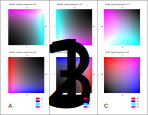
\includegraphics[width=\linewidth]{./images/expressions_fig.png}
\caption{Simulated retinal and tectal signalling molecule expression.
\textbf{A} A schematic of retino-tectal mapping.
%
\textbf{B} Retinal receptor expression, $r_i$. Four receptors are expressed and displayed here in two dual-colour maps. $r_0$ and $r_1$ are red and blue; $r_2$ and $r_3$ are cyan and magenta. $r_0$ increases as an exponential function of $-x$; $r_1$ increases with an exponential function of $-y$. $r_2$ and $r_3$ have the opposite sense. Retinal receptor expression is modelled with exponential functions because there is ample evidence to support this form. $N$: nasal, $T$: temporal, $D$: dorsal, $V$: ventral.
%
\textbf{C} Retinal ligand expression, $l_i$, is expressed in complimentary gradients \citep{hornberger_modulation_1999}.
%
\textbf{D} Tectal ligand expression $L_i$. Tectal ligand expression is shown in an exponential form, although there is less evidence to determine whether tectal expression is exponential, linear or logarithmic.
$L$: lateral, $M$: medial, $C$: caudal, $R$: rostral.
}
\label{f:ex}
\end{figure}

% FIGURE 2
\begin{figure}
\includegraphics[width=\linewidth]{./images/j4_ee_GJ_best_1_wt_fig2_exit_true_steps_1500.png}
\caption{Receptor-ligand model of chemotaxis and competition.
\textbf{A} The origin position on the retina gives axons a colour according to a dual-colour map. Axons in panels B-H that are red are those which originated in the most naso-ventral corner of the square simulated retina.
\textbf{B}-\textbf{D} Axon centroid positions on the simulated tectum (dashed line) at time 0, 40 and 1500 units. Lines show adjacency relationships between the axons' origin positions on the retina.
\textbf{E} Layout of axon centroids on the tectum observed in experimental results \textbf{expectation or prediction}.
\textbf{F} The sum-of-squared difference error, $\epsilon$, and the number-of-crossings error metric, $\eta$ of the tectal axon arrangement plotted with respect to simulation time. \textbf{two subgraphs better}
\textbf{G} The arrangement of axon branches at t=1500.
\textbf{H} Selected axon locations at t=1500, with path histories in grey.
\emph{Abbreviations: D dorsal, V ventral, T temporal, N nasal, C caudal, R rostral, M medial, L lateral.}}
\label{f:GJ}
\end{figure}

% FIGURE 3 ./scripts/fig_GJ_surgical.sh
% Could split into retina and tectum or
% a: rotation/graft (as hand waved by Gierer)
% b: ablation (as simulated in 1D by Gierer)
% c: mismatch/compound (as extensions of Gierer)
\begin{figure}
{\centering

\includegraphics[width=0.75\linewidth]{./images/fig_GJ_surgical.png}
\par }
\caption{Performance of the model with surgical manipulations. Here, we made a number of simulated surgical manipulations of the tectum and retina and applied the same model shown in Fig\,\ref{f:GJ}. \textbf{A.} Graft rotation. An 8$\times$8 square patch of tectum has been rotated by 90$\degree$, altering the tectal ligand expression pattern. High gradients form around the new discontinuities at the edge of the patch (see Fig\,\ref{f:trot90}), driving axons to follow the rotation of the patch. The left graph shows the axon centroid positions after 1500 time steps, the smaller inset graph shows the (idealised) anticipated layout seen in experiments \citep{levine_deployment_1974}. The right-hand graph shows the time-course of the pattern quality metric, $\epsilon$ (i.e.~how closely the centroid pattern matches the inset) for the entire tectum (blue), the graft region (yellow) and the surround (red). The axons within the graft are slightly less well ordered than those outside. \textbf{B} Shows the same type of graft rotation as \textbf{A} for a 180$\degree$ rotation \citep{yoon_retention_1973}. \textbf{C.} A simulated graft swap experiment. Two 12$\times$4 rectangular regions of tectum are cut out and grafted back in swapped positions \citep{hope_arrow_1976,gaze_visuotectal_1983}. While there is disorder in the simulated pattern of axon centroids, a line of red/yellow agents that would been located caudally has advanced rostrally and a number of green agents are more caudal than in the wildtype arrangement. Note that here, the pattern metric shown for `Graft' (yellow curve) is computed from a square covering both grafts. \textbf{D.} The temporal half of the retina is removed in this manipulation. Axons from the nasal half grow onto an unmodified tectum. This manipulation is problematic for the pure chemoaffinity theory, because axons from the middle of the retina now grow towards the rostral side of the tectum; the topographic map of the remaining retina expands across the entire tectum. In this work, it is the competition that achieves this effect. In panels D-G, the axon centroid graphs are plotted as in A-C, but right hand graph indicates the rostro-caudal tectal position of each axon centroid as a function only of its naso-temporal origin on the retina. \textbf{E}. Axons from an unmanipulated retina grow onto a tectum whose caudal half has been removed. As in experiments \citep{yoon_reorganization_1971,finlay_orderly_1979}, the axons `crush up' to form a complete map of the retina over the half tectum. \textbf{F.} A `mismatch' experiment \citep{horder_retention_1971}. The axons from the surviving nasal half of an ablated retina, which would usually map to the caudal half of the tectum arrange themselves into a map on the \emph{rostral} half of the tectum as the caudal portion has been removed. As with the other ablations, the model achieves this due to variable interactions with the tectal ligand gradient and competitive interactions. \textbf{G} Compound eye. If two nasal retina halves are grafted together, two overlaid maps form on the tectum \citep{gaze_retino-tectal_1963}. The simulation reproduces this result because axons from corresponding locations on the naso-temporal retinal axis interact equally with the tectal gradients and arrive in similar locations.}
\label{f:GJsurg}
\end{figure}

% FIGURE 4
\begin{figure}
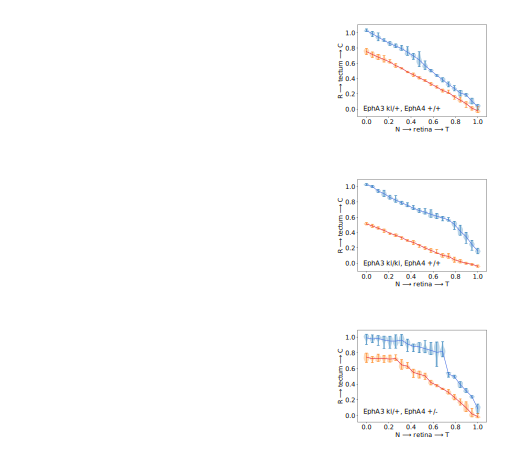
\includegraphics[width=0.95\linewidth]{./images/EphA_manipulations.png}
\caption{Three genetic manipulations simulating those performed by \citet{brown_topographic_2000} and \citet{reber_relative_2004}. In each manipulation, the left graph shows axon branch agents at the end of a simulation ($t=1500$), the centre graph shows axon centroids (also at simulation end), with the colour blue indicating axons with no selective manipulation and red indicating those axons with a selective genetic knock-in of EphA3. In the right hand graph, the final rostro-caudal locations on the tectum of axons from each naso-temporal origin in the retina are plotted as violin plots (with bars indicating the maximum and minimum datum in each group and shading indicating the data distribution). Inset graphs show experimental results from  \citet{brown_topographic_2000} and \citet{reber_relative_2004}. \textbf{A} We simulated the heterozygous EphA3 knock-in (EphA3 ki/+) of \citet{brown_topographic_2000} by selecting half of the retinal cells at random, and in these cells adding the value 0.8 to $r_0$ (which, as its expression increases towards the temporal retina, is our analogue for EphA). The affected cells experienced altered interaction with tectal ligand gradients and were shifted rostrally. The rostral shift was largest for nasal cells bound for the caudal tectum. These experience the strongest interaction with $L_0$ (which is highest in caudal tectum). Temporal cells with the manipulation experience a smaller change in their final location because $L_0$ expression is low at their target location (and hence the $r_0$-$L_0$ interaction is minimal here). However, there is no evidence of the observed map collapse at around 0.8 on the N--T axis. \textbf{B} To increase the magnitude of the manipulation of EphA3, \citet{brown_topographic_2000} added a homozygous EphA3 knock-in (modelled as a knock-in of 3.2) which pushed manipulated cells further towards the rostral tectum. Here, we observed a separation into two maps, one for the wildtype cells and one for the manipulated cells, in agreement with \citet{brown_topographic_2000} (inset is from their Fig.\,5C). \textbf{C} Simulation of EphA3 ki/+ selective knock-in and EphA4 knock-down (all cells) from \citet{reber_relative_2004}. The knock-down was applied by reducing $r_0$ in all cells by 1.2. The system fails to reproduce either the map collapse at around 0.9 on the N--T axis, nor the strong rostral pull for selective knock-in cells seen in the experimental result. In fact, the selective knock-in cells are drawn in the \emph{caudal} direction, because the knock-down of 1.2 undoes the effect of the knock-in of 0.8.}
\label{f:GJeph}
\end{figure}

% FIGURE 5
\begin{figure}
\includegraphics[width=0.95\linewidth]{./images/EphA_manipulations_explanation.png}
\caption{Two new mechanisms to account for the genetic manipulation results: cluster-size and $r_2$ collapse. To account for map collapse (\citet{brown_topographic_2000} and Fig.\,\ref{f:GJeph}A), and the significant rostral termination of knock-in/knock-down cells (\citet{reber_relative_2004} and Fig.\,\ref{f:GJeph}C), we assumed that i) retinal EphA interactions with tectal ephrin ligands are modulated by EphA4 receptors through a `side-binding' mechanism and ii) EphA3 and EphA4 receptors interact with the receptors which mediate the chemotaxis effect that \emph{opposes} EphA ($r_2$). \textbf{A} As described in the text, EphA ($r_0$) is expressed according to $1.05 + 0.26 \exp(2.3 u)$ (green curve) where $u$ is the N--T retinal position in this case. Knock-in is simulated simply by adding 0.8 to this function (giving the purple curve). Retinal ephrinA expression is a reversed version of EphA expression (green dotted curve). \textbf{B} EphA4 expression is a new feature in this model extension. Overall EphA4 expression across the retina is constant (green dotted line, value 3.5) but retinal ephrinA can bind to EphA4, modelled here as a multiplicative interaction to give cis-bound EphA4 (green dashed curve) and un-bound EphA4 (green solid curve). We model genetic knock-down of EphA4 by subtracting a value of 2.1 from the constant EphA4 value, and re-apply the multiplication by retinal ephrinA to give the cyan curves. \textbf{NB: curves not quite right here - there should be a crossover of the filled cyan curve and the dotted red threshold near the T side; this is what happens in the sim. This it's due to an off-by-one discrepancy in x position.} \textbf{C} The signal strength, $s_0$, for an interaction between EphA receptors and a tectal ligand gradient is modelled as $s_0 = r_0 \times c_0$ where $c_0$, the cluster size, is $1/r_{A4}$. Shown for wildtype, knock-in and knock-down experiments, the cluster-size modulated signal $s_0$ increases for knock-in and for knock-down manipulations and is further enhanced with a combination of both knock-in and knock-down. \textbf{D} We assume that the strength of receptor interactions for $r_2$ collapses under the conditions that $r_0$ exceeds a threshold $h_0=1.6$ (red dotted line in A) and that $r_{A4}$ is simultaneously below a threshold $h_{A4}=1.1626$ (red dotted line in B). Under these conditions, $r_2$ is reduced to one fifth of its normal value. \textbf{Note for Stuart: The graphs are as-generated by a Python script. I'll fix the legend boxes etc once they are final.}}
\label{f:clustermech}
\end{figure}

%%% Caption for clustermechsize only model: \textbf{B} Model results. i) EphA3 knock-in result for ki=1.0. Inset shows experimental results from Fig.\,5B of \citet{brown_topographic_2000}. The graph appears similar to that in Fig.\,\ref{f:GJeph}A but crucially, the distributions of tectal locations begin to overlap at about 80\% of the N--T axis, in agreement with experiment. ii) The double knock-in result (Fig.\,5C of \citet{brown_topographic_2000}) agrees well with the experimental result, showing two, separated maps iii) When EphA is knocked in and EphA4 is simultaneously knocked-down, nasal axons experience an enhanced signal to move along gradients towards rostral tectum and so the red curve is drawn further rostrally. Although less dramatic than the experimental result of \citet{reber_relative_2004} the movement is in the correct direction, and the overlap of positions (the `collapse point') moves to about 90\% of the N--T axis. iv) Uniform knock-down of EphA4 in all cells does not perturb the mapping.

% FIGURE 6
\begin{figure}
\includegraphics[width=0.95\linewidth]{./images/EphA_manipulations_clustertheory_r2collapse.png}
\caption{Model results with the mechanisms described in Fig.\,\ref{f:clustermech}. \textbf{A} EphA3 knock-in result for ki=0.8. The graph appears similar to that in Fig.\,\ref{f:GJeph}A but crucially, the distributions of tectal locations begin to overlap at about 80\% of the N--T axis, in agreement with experiment \textbf{Seb to check stats on this}. \textbf{B} The double knock-in result shows excellent agreement with the experimental result. \textbf{C} When EphA is knocked in and EphA4 is simultaneously knocked-down, nasal axons experience an enhanced signal to move along gradients towards rostral tectum and so the red curve is drawn further rostrally. Additionally, the combined knock-in and knock-down triggers the $r_2$ receptors to become one fifth as effective, leading to a degraded signal to move along gradients towards the caudal tectum. Consequently, the red curve is moved much more caudally, in agreement with \citet{reber_relative_2004}. \textbf{D} Uniform knock-down of EphA4 in all cells does not perturb the mapping to a significant extent. \textbf{TODO: Answer question as to why this curve is drawn rostrally and describe the discontinuity at 0.25 on N--T axis, at which the collapse mechanism is being engaged. Need to figure out the slight discrepancy between signals in Fig.\,\ref{f:clustermech} and those in the simulation.}}
\label{f:r2collapse}
\end{figure}

% ANY SUPPLEMENTARY FIGURES GO AFTER THIS
%\renewcommand{\thefigure}{S\arabic{figure}}
%\setcounter{figure}{0}

% FIGURE S1
\begin{figure}
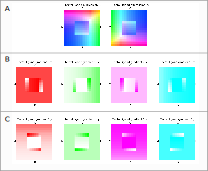
\includegraphics[width=\linewidth]{./images/Tissuevisb.png}
\caption{(Supplementary) Ligand expression and gradients on the tectum for the
graft-rotate 90 degrees simulated surgical manipulation}
\label{f:trot90}
\end{figure}

% DITCH THIS ONE
%
% FIGURE S2
%%\begin{figure}
%%\includegraphics[width=\linewidth]{./images/j4_ee_G_wt_fig2_exit_true.png}
%%% Note MANUAL reference to Fig. 2 here (otherwise it says Fig S2):
%%\caption{Receptor-ligand model of chemotaxis alone. Panels A-H show results as in Fig\,\textbf{2}. Briefly:
%%\textbf{A} Retinal cell position colour scheme.
%%\textbf{B}-\textbf{D} Axon centroid positions on the simulated tectum (dashed line) at time 0, 40 and 1500 units. In this chemotaxis-only model, which differs from that shown in Fig\,\ref{f:GJ} only by having the parameter $m_X$ set to 0 in Eq.\,\ref{e:X}, variable interactions with the gradients cause each RGC to find a location that preserves the topographic ordering, but the absence of competition means that axons fail to extend across the full tectum.
%%\textbf{E} Anticipated layout.
%%\textbf{F} The sum-of-squared difference error, $\epsilon$, and the number-of-crossings error metric, $\eta$ of the tectal axon arrangement plotted with respect to simulation time.
%%\textbf{G} The arrangement of axon branches at t=1500.
%%\textbf{H} Selected axon locations at t=1500, with path histories in grey.
%%\emph{Abbreviations: D dorsal, V ventral, T temporal, N nasal, C caudal, R rostral, M medial, L lateral.}}
%%\label{f:G}
%%\end{figure}

\end{document}
